% (c) 2002 Matthew Boedicker <mboedick@mboedick.org> (original author) http://mboedick.org
% (c) 2003-2007 David J. Grant <davidgrant-at-gmail.com> http://www.davidgrant.ca
% (c) 2008 Nathaniel Johnston <nathaniel@nathanieljohnston.com> http://www.nathanieljohnston.com
% (c) 2011 Scott Clark <sc932@cornell.edu> http://cam.cornell.edu/~sc932
% (c) 2022 Arne Hassel <arne.hassel@gmail.com> http://icanhasweb.net/
%
% This work is licensed under the Creative Commons Attribution-Noncommercial-Share Alike 2.5 License. To view a copy of this license, visit
% http://creativecommons.org/licenses/by-nc-sa/2.5/ or send a letter to Creative Commons, 543 Howard Street, 5th Floor, San Francisco, California, 94105, USA.

\documentclass[letterpaper,10pt,norsk]{article}
\newlength{\outerbordwidth}
\pagestyle{empty}
\raggedbottom
\raggedright
\usepackage{babel}
\usepackage{float}
\usepackage[T1]{fontenc}
\usepackage{framed}
\usepackage{graphicx}
\usepackage{hyperref}
\usepackage[utf8]{inputenc}
\usepackage{tocloft}
\usepackage{url}
\usepackage[svgnames]{xcolor}
\usepackage{wrapfig}
\usepackage{tabularx}

%-----------------------------------------------------------

% Edit these values as you see fit

\setlength{\outerbordwidth}{2pt}  % Width of border outside of title bars
\definecolor{shadecolor}{gray}{0.75}  % Outer background color of title bars (0 = black, 1 = white)
\definecolor{shadecolorB}{gray}{0.93}  % Inner background color of title bars

%-----------------------------------------------------------

% Margin setup

\setlength{\evensidemargin}{-0.25in}
\setlength{\headheight}{-0.25in}
\setlength{\headsep}{0in}
\setlength{\oddsidemargin}{-0.25in}
\setlength{\paperheight}{11in}
\setlength{\paperwidth}{8.5in}
\setlength{\tabcolsep}{0in}
\setlength{\textheight}{9.75in}
\setlength{\textwidth}{7in}
\setlength{\topmargin}{0in}
\setlength{\topskip}{0in}
\setlength{\voffset}{0.1in}

%-----------------------------------------------------------

% Custom commands

\newcommand{\resitem}[1]{\item #1 \vspace{-2pt}}

\newcommand{\resheading}[1]{\vspace{8pt}
\parbox{\textwidth}{\setlength{\FrameSep}{\outerbordwidth}
  \begin{shaded}
    \setlength{\fboxsep}{0pt}\framebox[\textwidth][l]{\setlength{\fboxsep}{4pt}\fcolorbox{shadecolorB}{shadecolorB}{\textbf{\sffamily{\mbox{~}\makebox[6.762in][l]{\large #1} \vphantom{p\^{E}}}}}}
  \end{shaded}
}\vspace{-5pt}
}

\newcommand{\ressubheading}[4]{
  \begin{tabularx}{6.5in}{l@{\cftdotfill{\cftsecdotsep}\extracolsep{\fill}}r}
    \textbf{#1} & #2          \\
    \textit{#3} & \textit{#4} \\
  \end{tabularx}
  \vspace{-6pt}
}

%-----------------------------------------------------------

\title{Curriculum Vitae}

\begin{document}

  \begin{minipage}{\textwidth}
    \begin{wrapfigure}{r}{0pt}
      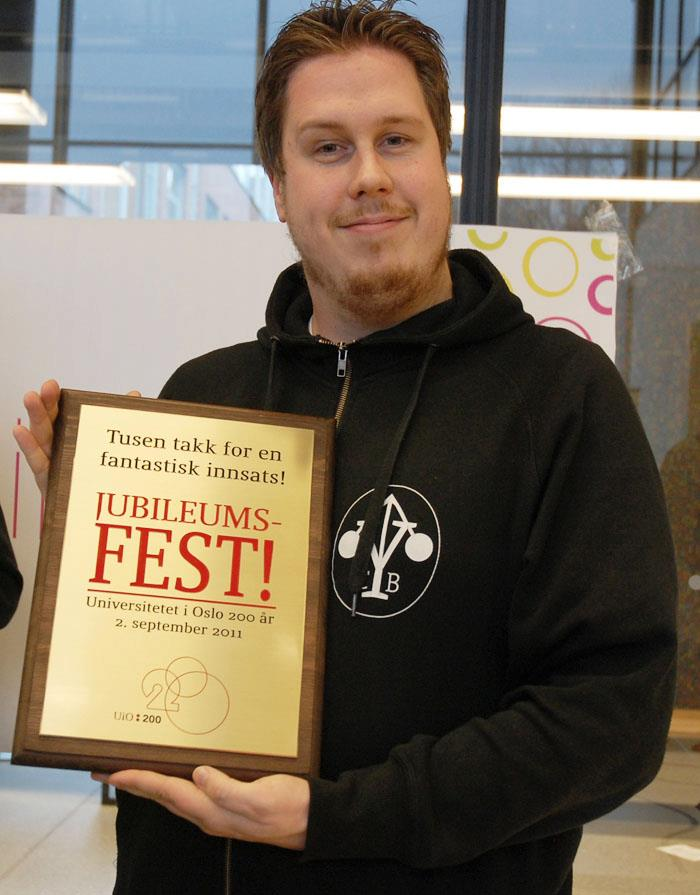
\includegraphics[height=45mm]{uio200.jpg}
    \end{wrapfigure}

    \textbf{\Large Curriculum Vitae for Arne Hassel}

    \vspace{5mm}

    \begin{tabular}{p{1in} l}
      Adresse:     & Helgesens gate 12 F, 0553 Oslo \\
      Telefon:     & 416 94 086                     \\
      E-post:      & \url{arne.hassel@gmail.com}    \\
      Født:        & 5. desember 1984               \\
      Sivilstatus: & Ugift                          \\
    \end{tabular}

    \vspace{5mm}

    \begin{minipage}{5.5in}
      Front-end utvikler med lang erfaring innenfor web-utvikling, med master i informatikk og bachelor i økonomi og administrasjon. Jeg er veldig glad i
      jobbe med nettbaserte teknologier som HTML, CSS, TypeScript, og \href{https://www.w3.org/standards/semanticweb/data}{Linked Data}. Jeg er veldig flink
      til å jobbe i team og sørger for at alt jeg leverer er tilgjengelig og respekterer alle involverte brukergrupper. Jeg er også en sterk pådriver for hva
      Linked Data kan gjøre for tjenester og sluttbrukere. Trives også i rollen som mentor for utviklere, og har fått gode tilbakemeldinger på min
      tålmodighet og evne til å svare på spørsmål.
    \end{minipage}

  \end{minipage}

  \resheading{Arbeidserfaring}

  \begin{itemize}
    \item
    \ressubheading{Inrupt}{Oslo}{Senior front-end utvikler}{2018 - 2022}
    \begin{itemize}
      \item Jobbet med flere applikasjoner knyttet til \href{https://solidproject.org/}{prosjektet Solid}, hvor jeg også hadde æren av å jobbe med
      \href{https://en.wikipedia.org/wiki/Tim_Berners-Lee}{Tim Berners-Lee}. Jobbet mye med React.
    \end{itemize}
    \item
    \ressubheading{Bouvet ASA}{Oslo}{Senior front-end utvikler}{2017 - 2019}
    \begin{itemize}
      \item Jobbet hos Tine og Arkivverket som frontend tech lead, brukte mye \href{https://enonic.com/resources/enonic-xp-all-you-need-to-know}{Enonic XP}
      og React.
    \end{itemize}
    \item
    \ressubheading{Questback AS}{Oslo}{Front-end utvikler}{2014 - 2017}
    \begin{itemize}
      \item Ansvarlig for front-end utviklingen av et produkt. Teknologier mye brukt er Angular, Grunt, Knockout, og jQuery.
    \end{itemize}
    \item
    \ressubheading{Senter for pasientmedvirkning og samhandlingsforskning}{Oslo}{Systemutvikler}{2008 - 2014}
    \item
    \ressubheading{Kiwi}{Risør \& Oslo}{Deltidsmedarbeider}{1999 - 2008}
    \item
    \ressubheading{Senter for Helse \& Arbeid}{Oslo}{Personlig assistent}{2008}
  \end{itemize}

  \resheading{Utdanning}

  \begin{itemize}
    \item
    \ressubheading{Institutt for informatikk, Universitetet i Oslo}{Oslo}{Master i informatikk: programmering og nettverk}{2010 - 2012}
    \begin{itemize}
      \item Skrev masteroppgave om JavaScript og Semantisk Web, veiledere var Kjetil Kjernsmo og Martin Giese
    \end{itemize}
    \item
    \ressubheading{Institutt for informatikk, Universitetet i Oslo}{Oslo}{Profesjonsstudie, Distribuerte Systemer og Nettverk}{2007 - 2010}
    \item
    \ressubheading{Universitetet for miljø og biovitenskap}{Ås}{Bachelor i økonomi og administrasjon}{2003 - 2007}
    \item
    \ressubheading{Risør VGS}{Risør}{Allmenne fag}{2000 - 2003}
  \end{itemize}

  \resheading{Sertifiseringer \& ferdigheter}

  Se vedlagt kompetansediagram for ytterligere detaljer.

  \begin{itemize}
    \item MS: Programming in HTML5 with JavaScript and CSS3 (Microsoft, 2015)
    \item MCPS: Microsoft Certified Professional (Microsoft, 2015)
    \item Certified ScrumMaster (Scrum Alliance, 2013-2015)
  \end{itemize}

  \resheading{Utvalgte prosjekter}

  \begin{itemize}
    \item {\bf Ifi-ordenen nettside:} Nettside med Next/React og Sanity. Utviklet sammen med designere for å gjøre nettsiden mer tilgjengelig for
    studenter.
    \url{https://ordenen.ifi.uio.no/}
    \item {\bf CYB50 nettside:} La ut jubileumsboken som jeg var redaktør for i nettside-format. Brukte Gatsby/React og MDX-filer for innhold.
    \url{https://50.cyb.no/}
  \end{itemize}

  \resheading{Frivillig arbeid og tillitsverv}

  \begin{itemize}
    \item
    \ressubheading{Solid}{Oslo}{Frivillig}{2018 - nåværende}
    \item
    \ressubheading{CYB50 Jubileumsbok}{Oslo}{Redaktør}{2018-2019}
    \item
    \ressubheading{Hennes Majestet Keiserpingvinen den Fornemmes orden}{Oslo}{Stormester}{2014 - nåværende}
    \item
    \ressubheading{Holder de ord}{Oslo}{Programmerer}{2012 - 2018}
    \item
    \ressubheading{Kodeklubben Oslo}{Oslo}{Kodeveileder}{2015 - 2016}
    \item
    \ressubheading{Cybernetisk Selskab (CYB)}{Oslo}{Kasserer, økonomifunksjonær, fadderstyremedlem, vakt}{2009 - 2011}
    \item
    \ressubheading{Bursdagsfesten på Ole-Johan Dahls hus 2. september}{Oslo}{Festgeneral/Koordinator}{2011}
    \item
    \ressubheading{IAESTE}{Ås}{Dataansvarlig, leder, økonomiansvalig, nestleder}{2003 - 2007}
  \end{itemize}

  \resheading{Personlige detaljer}

  \begin{itemize}
    \item {\bf Hobbyer:} Lese, lage musikk
    \item Har førerkort klasse B
  \end{itemize}

  \resheading{Referanser}

  Jeg vil oversende en liste med mine referanser om dette skulle bli aktuelt.

\end{document}
